\documentclass[a4paper,11pt]{article}
\usepackage{graphicx,url}
\usepackage[T1]{fontenc}
\usepackage[utf8]{inputenc}
\usepackage[brazil]{babel}
\usepackage{a4wide}
\graphicspath{{./imagens/}}
\title{\vspace{-4cm}Relatório 03 - Laboratório de Arquitetura de Computadores}
\author{Luiz Junio Veloso Dos Santos - Matricula: 624037}

\begin{document} 

\maketitle

        \begin{figure}[ht]
            \caption{ALU de 4 bits}
            \centering
            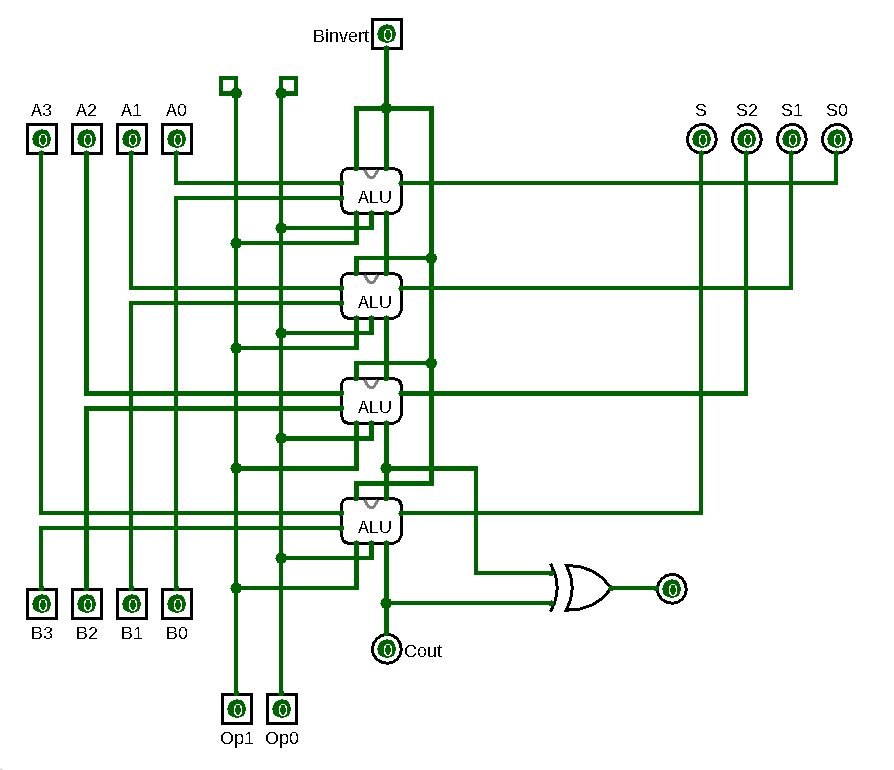
\includegraphics[width=12cm]{ALU4}
        \end{figure}
        \begin{figure}[ht]
            \caption{ALU de 1 bit}
            \centering
            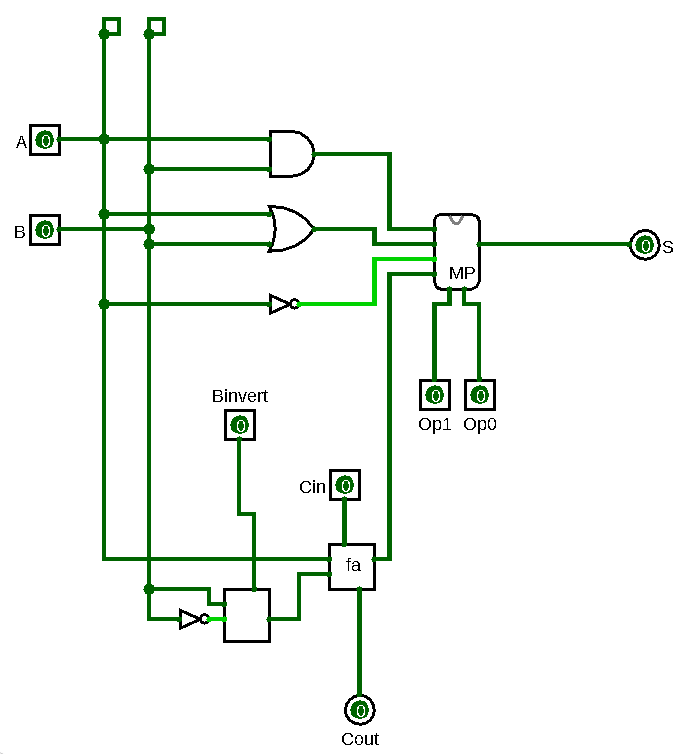
\includegraphics[width=10cm]{ALU}
        \end{figure}
        \begin{figure}[ht]
            \caption{Multiplexador 4x1}
            \centering
            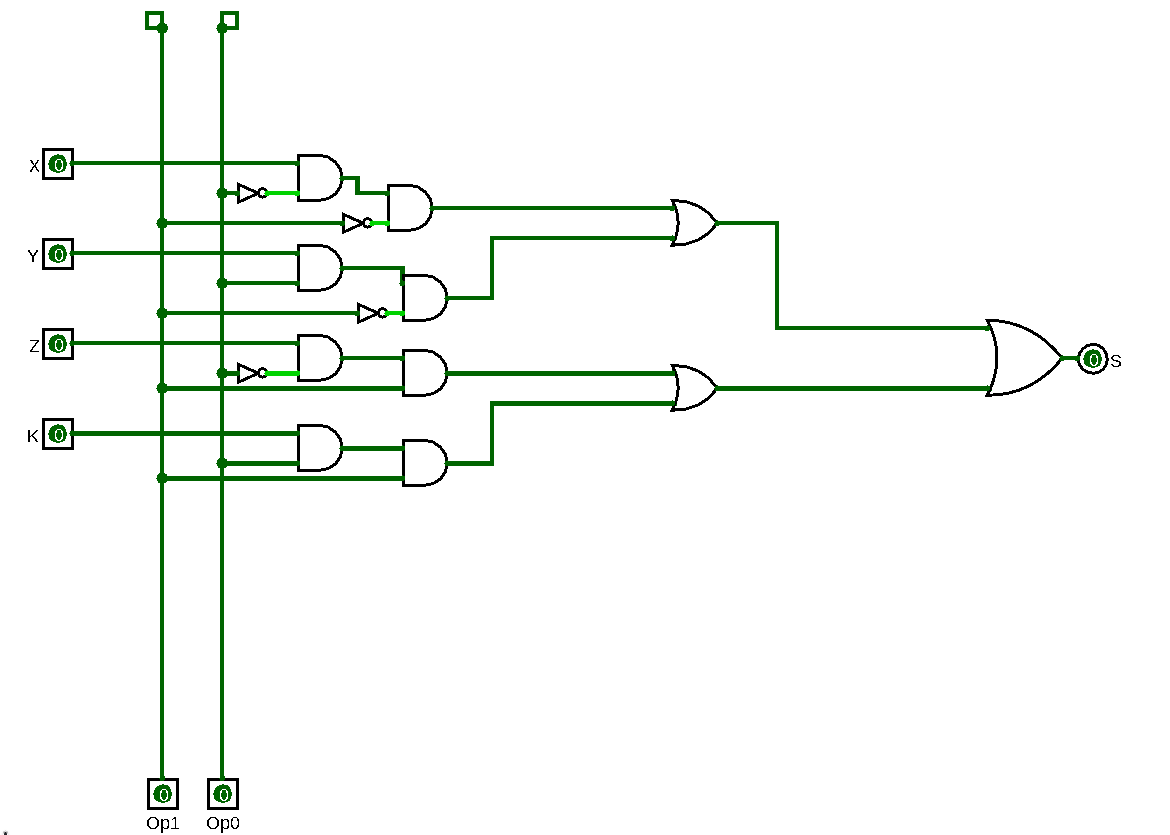
\includegraphics[width=10cm]{mux4}
        \end{figure}     
        \begin{figure}[ht]
            \caption{Multiplexador 2x1}
            \centering
            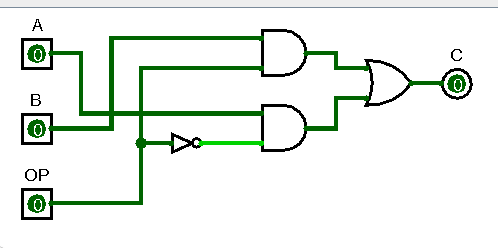
\includegraphics[width=10cm]{mux2}
        \end{figure}       
        \begin{figure}[ht]
            \caption{Full adder}
            \centering
            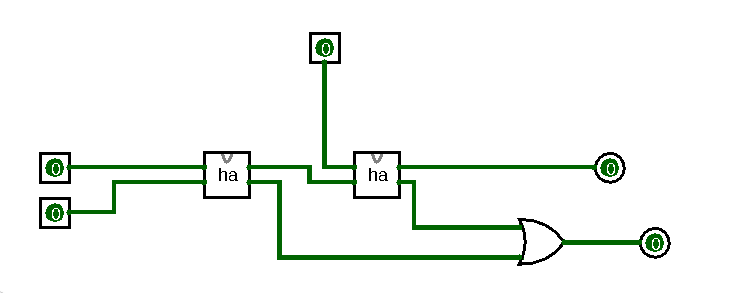
\includegraphics[width=10cm]{fulladder}
        \end{figure}       
        \begin{figure}[ht]
            \caption{Half adder}
            \centering
            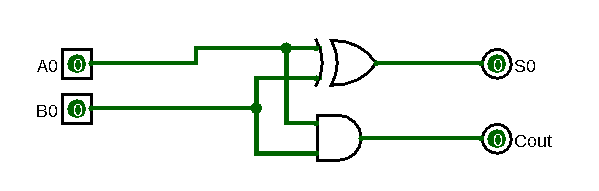
\includegraphics[width=10cm]{halfadder}
        \end{figure}
        \begin{figure}[ht]
            \caption{Parte 2 - and(a,b)}
            \centering
            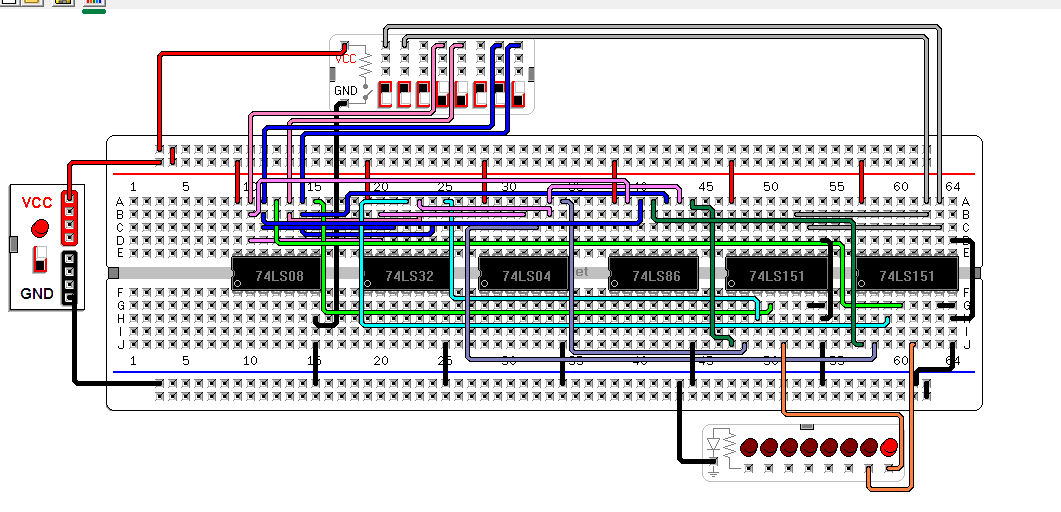
\includegraphics[width=16cm]{and}
        \end{figure}                   
        \begin{figure}[ht]
            \caption{Parte 2 - or(a,b)}
            \centering
            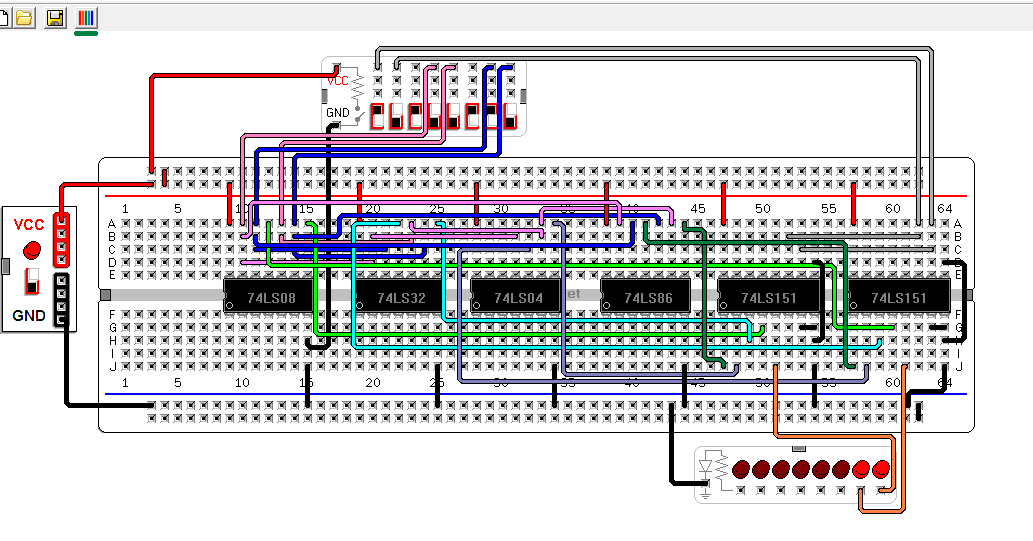
\includegraphics[width=16cm]{or}
        \end{figure}                                 
        \begin{figure}[ht]
            \caption{Parte 2 - soma(a,b)}
            \centering
            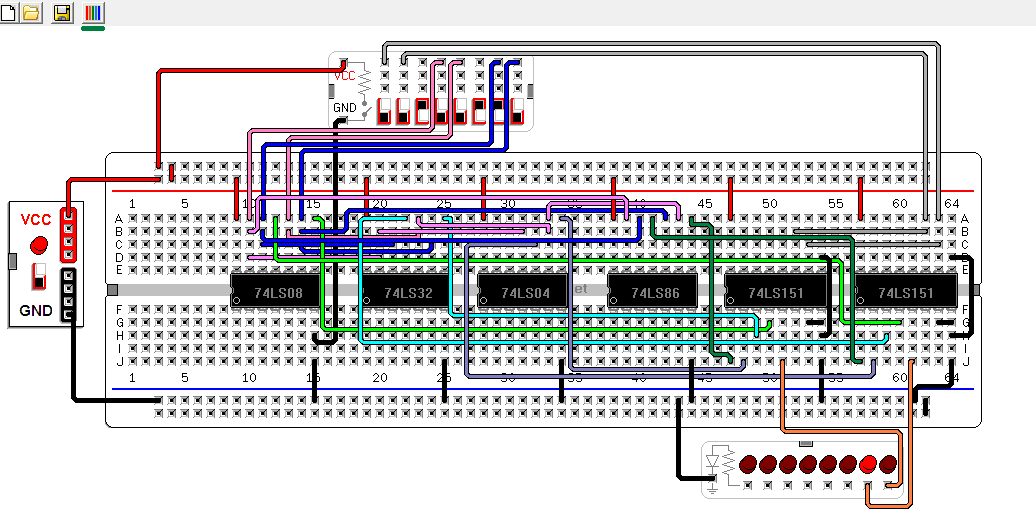
\includegraphics[width=16cm]{soma}
        \end{figure}                         
        \begin{figure}[ht]
            \caption{Parte 2 - not(a)}
            \centering
            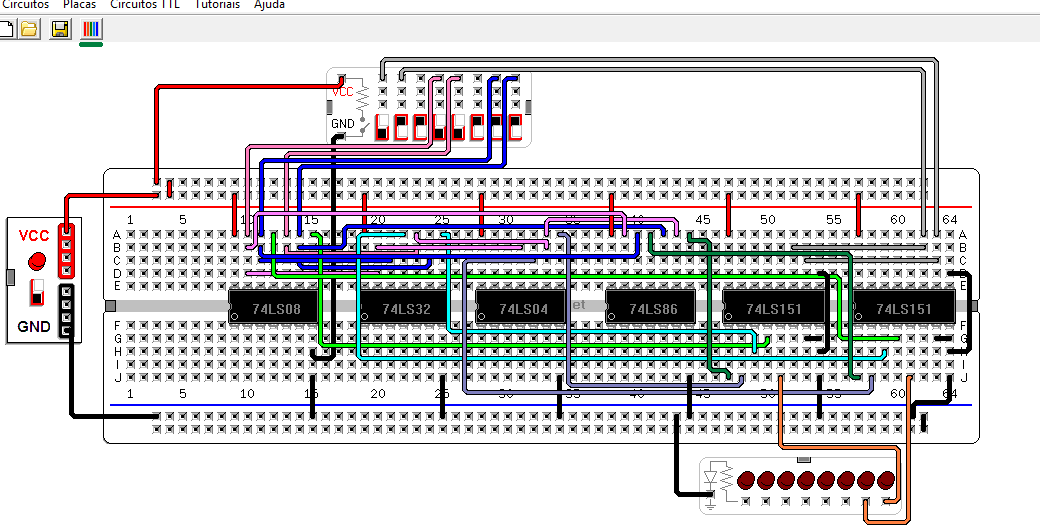
\includegraphics[width=16cm]{not}
        \end{figure}                         
        \begin{figure}[ht]
            \caption{Parte 2 - and(b,a)}
            \centering
            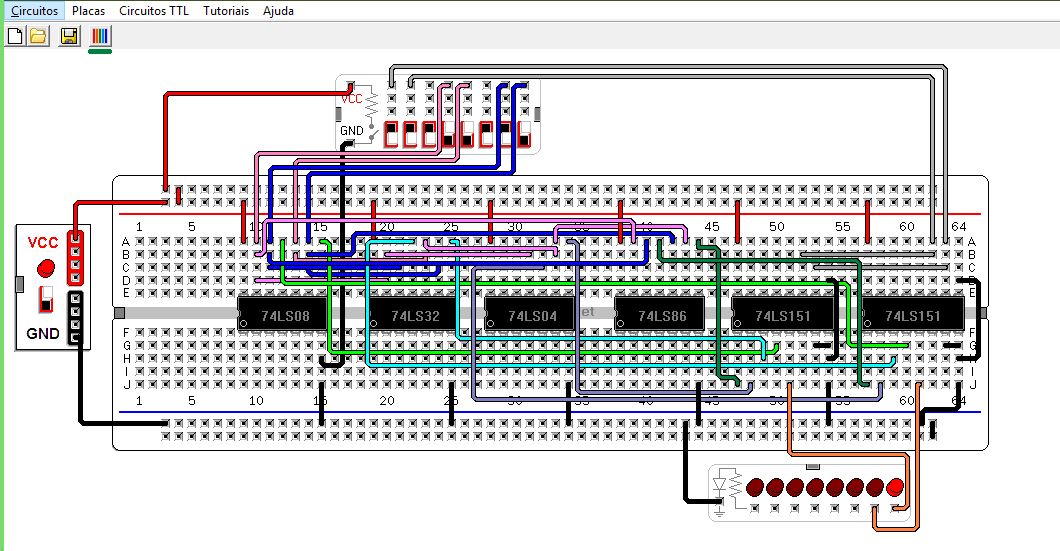
\includegraphics[width=16cm]{and2}
        \end{figure}                         
\end{document}
